\documentclass{book}

\usepackage{float} % Required for specifying the exact location of a figure or table
\usepackage{graphicx} % Required for including images
\usepackage{wrapfig}
\usepackage{standalone}
\newcommand{\HRule}{\rule{\linewidth}{0.5mm}} % Command to make the lines in the title page
\graphicspath{ {.././source/} }

\setlength\parindent{0pt} % Removes all indentation from paragraphs
%\setcounter{tocdepth}{2}


%----------------------------------------------------------------------------------------
%Title Page Defined with a horizontal line above and below
%\HRule \\[.4cm] \Huge \bfseries Allegan County GIS Services\\[0.5cm] \Large startup guide
%\title{\HRule \\[.4cm]\Huge \bfseries Policy
\title{\HRule \\[.4cm] 
\begin{figure}[H] % included image
\begin{center}	 
	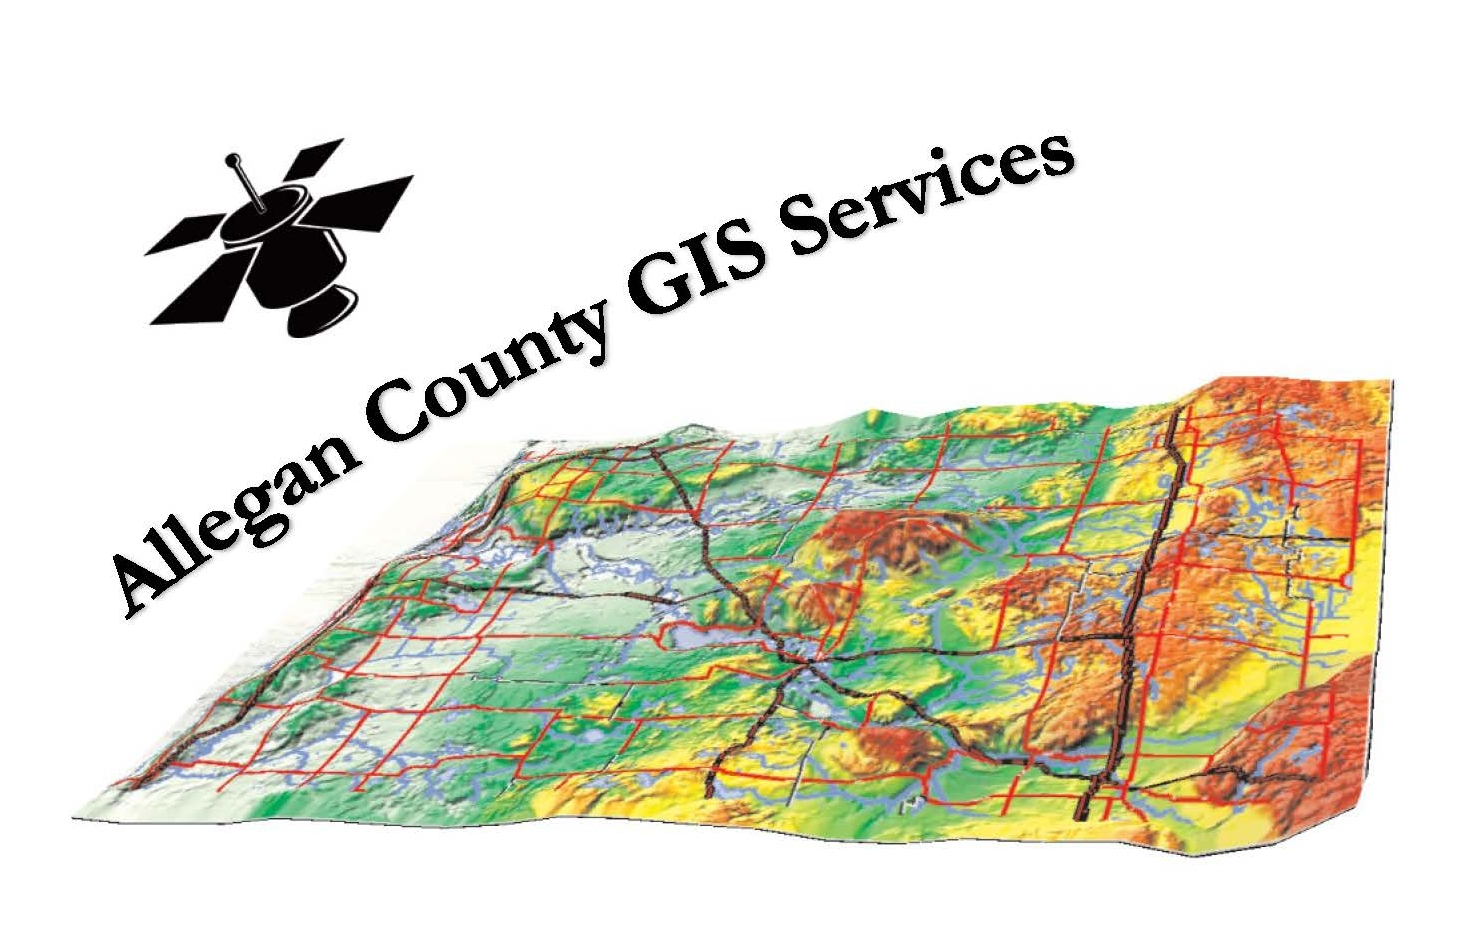
\includegraphics[scale=.5]{GIS_Logo_better.jpg}
	\end{center}
	\end{figure}
	\Huge \bfseries What We Do
\HRule \\[.4cm]
}

\author{\Large Allegan County GIS \\\Large www.allegancounty.org/gis}
%----------------------------------------------------------------------------------------

%Document Begins
\begin{document}
\frontmatter

%----------------------------------------------------------------------------------------
%%Title Page Called
\maketitle
%----------------------------------------------------------------------------------------
%\tableofcontents\clearpage
\tableofcontents
\mainmatter
\pagebreak
%----------------------------------------------------------------------------------------
\part*{Introduction}
\part{Goals}
\chapter{Goal X}
Description of goal X
\section{section}
Section about goal
\subsection{Subsection}
Further info
\subsubsection{subsubsection}
More info
\paragraph{paragraph about stuff}
paragraph text
\subparagraph{subparagraph about stuff}
subparagraph text

%----------------------------------------------------------------------------------------
\part{Methods}
\chapter{Method X}
Description of Method X
\section{section}
Section about Method
\subsection{Subsection}
Further info
\subsubsection{subsubsection}
More info
\paragraph{paragraph about stuff}
paragraph text
\subparagraph{subparagraph about stuff}
subparagraph text

%----------------------------------------------------------------------------------------
\part{Tangibles}

\chapter{Tools}

\documentclass{book}

\usepackage{float} % Required for specifying the exact location of a figure or table
\usepackage{graphicx} % Required for including images
\usepackage{wrapfig}
\newcommand{\HRule}{\rule{\linewidth}{0.5mm}} % Command to make the lines in the title page

\setlength\parindent{0pt} % Removes all indentation from paragraphs
%\setcounter{tocdepth}{2}
\graphicspath{ {.././source/} }

\begin{document}


\section{Using COGO Tools in QGIS}
%\pagebreak

\subsection{Set up the Azimuth and Distance Plugin \small(Azd Plugin).}
%\paragraph{After starting QGIS in the basemap}

\subsubsection{Launch Azd Plugin}
\large {In the Plugins drop down(1) under the topography group select the Azd Plugin(2)(see fig.).}
\begin{figure}[H] % included image
\begin{center}
%\centering
	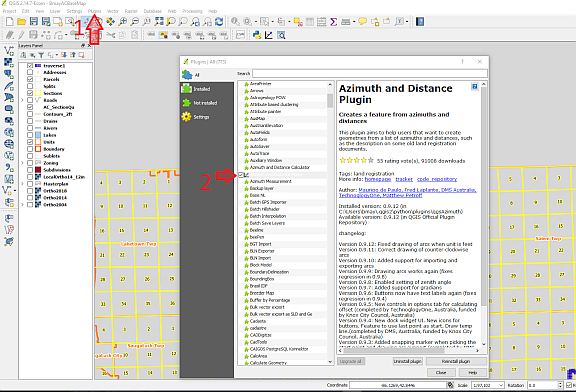
\includegraphics[scale=.25]{1.png}
	\end{center}
	\caption{launch plugin}	
\end{figure}
%\pagebreak
\clearpage

\subsubsection{Configure Active Layer}
\large Note here which layer is active.
\begin{figure}[H] % included image
\begin{center}
	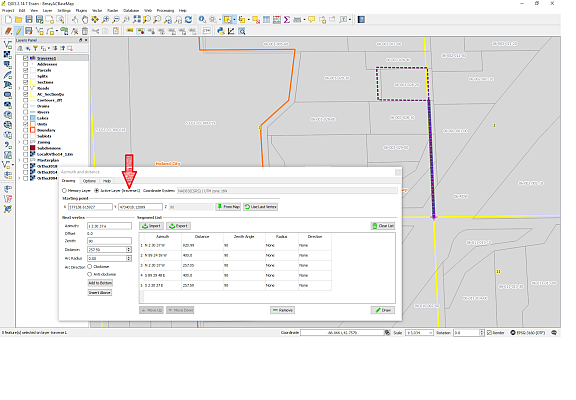
\includegraphics[scale=.2]{2.png} 
	\end{center}
	\caption{check active layer}
\end{figure}

%\noindent
If necessary, left click the layer traverse 1 in Layer Panel to activate it(see fig.).
\begin{figure}[H] % Example of including images
\begin{center}
	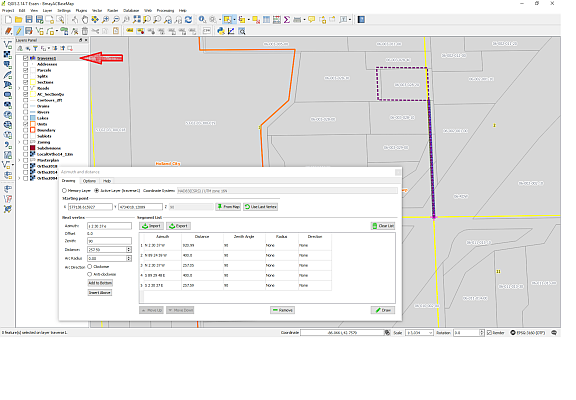
\includegraphics[scale=.2]{3.png} 
	\end{center}
	\caption{activate layer}
\end{figure}

\subsubsection{Configure Options}
\large On Options Tab: Select Boundary, Bearing, Feet, and Degree radio buttons.
\begin{figure}[H]
\begin{center}
	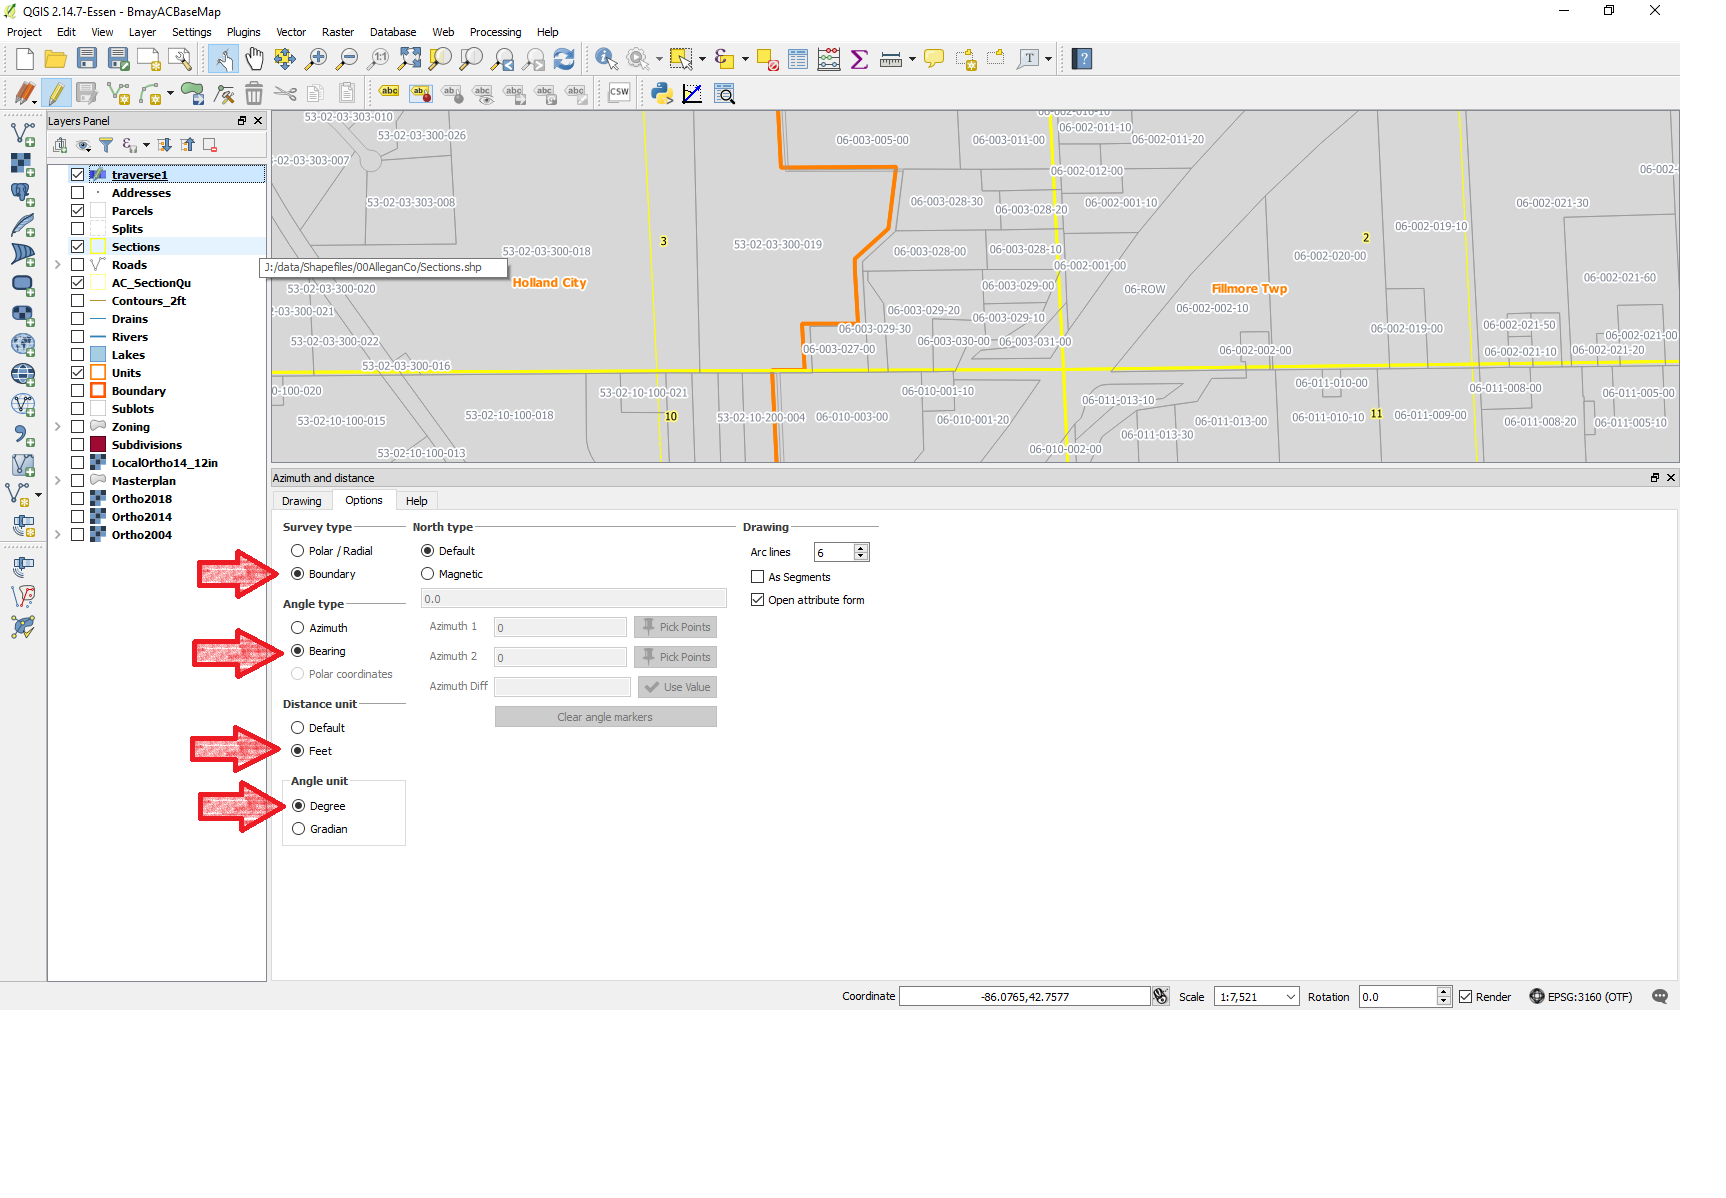
\includegraphics[scale=.3]{4.png} 
	\end{center}
	\caption{Plugin Options}
\end{figure}
\pagebreak

\subsubsection{Using the tool}
\large Boundary descriptions are entered into the Drawing Tab. Azimuth (bearing) and Distance are the important boxes (Set Offset = 0 and Zenith = 90 and ignore)(see below).
\begin{figure}[H]
\begin{center}
	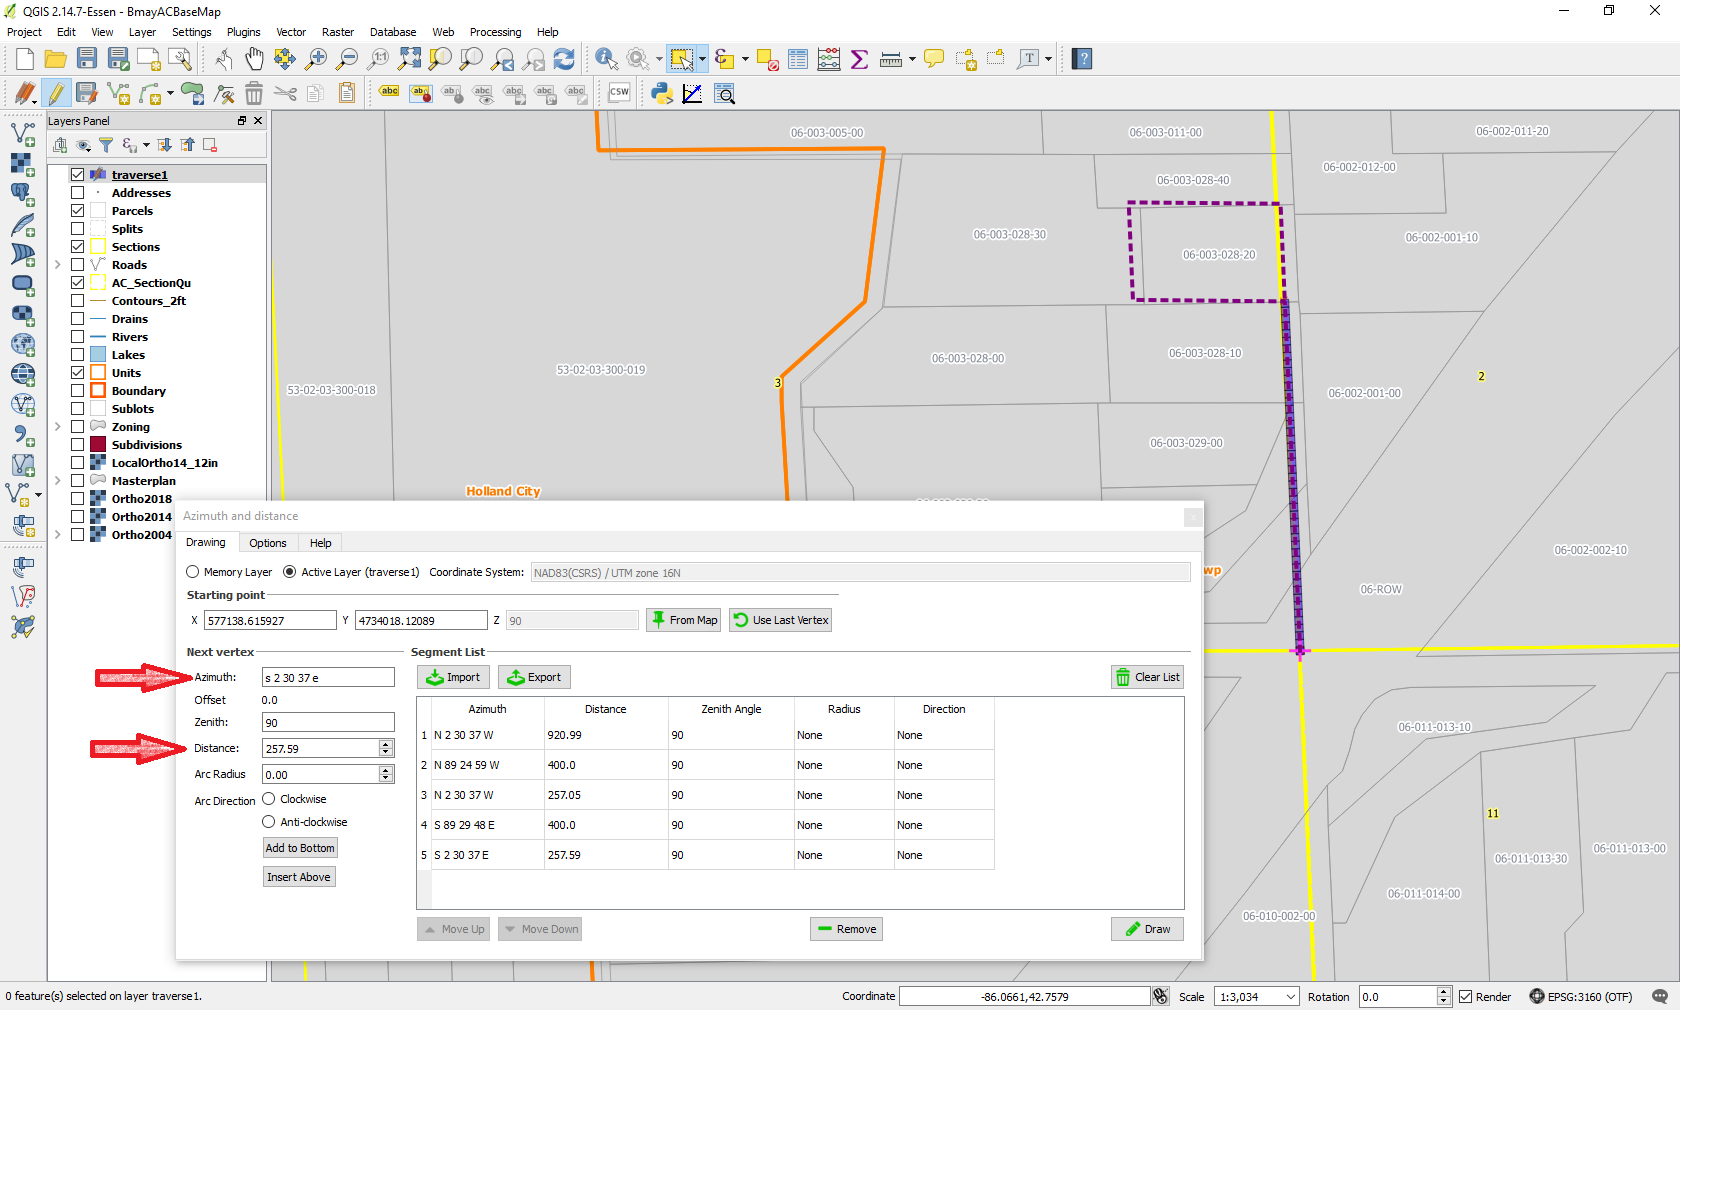
\includegraphics[scale=.3]{5.png} 
	\end{center}
	\caption{Entering Bounds}
\end{figure}
\pagebreak

\subsection{Configure editing environment}
\large Use Settings Dropdown and Snapping Options to enable snapping to Sections, Quarter Sections, and or Parcels if desired (see fig.).

\begin{figure}[H]
\begin{center}
	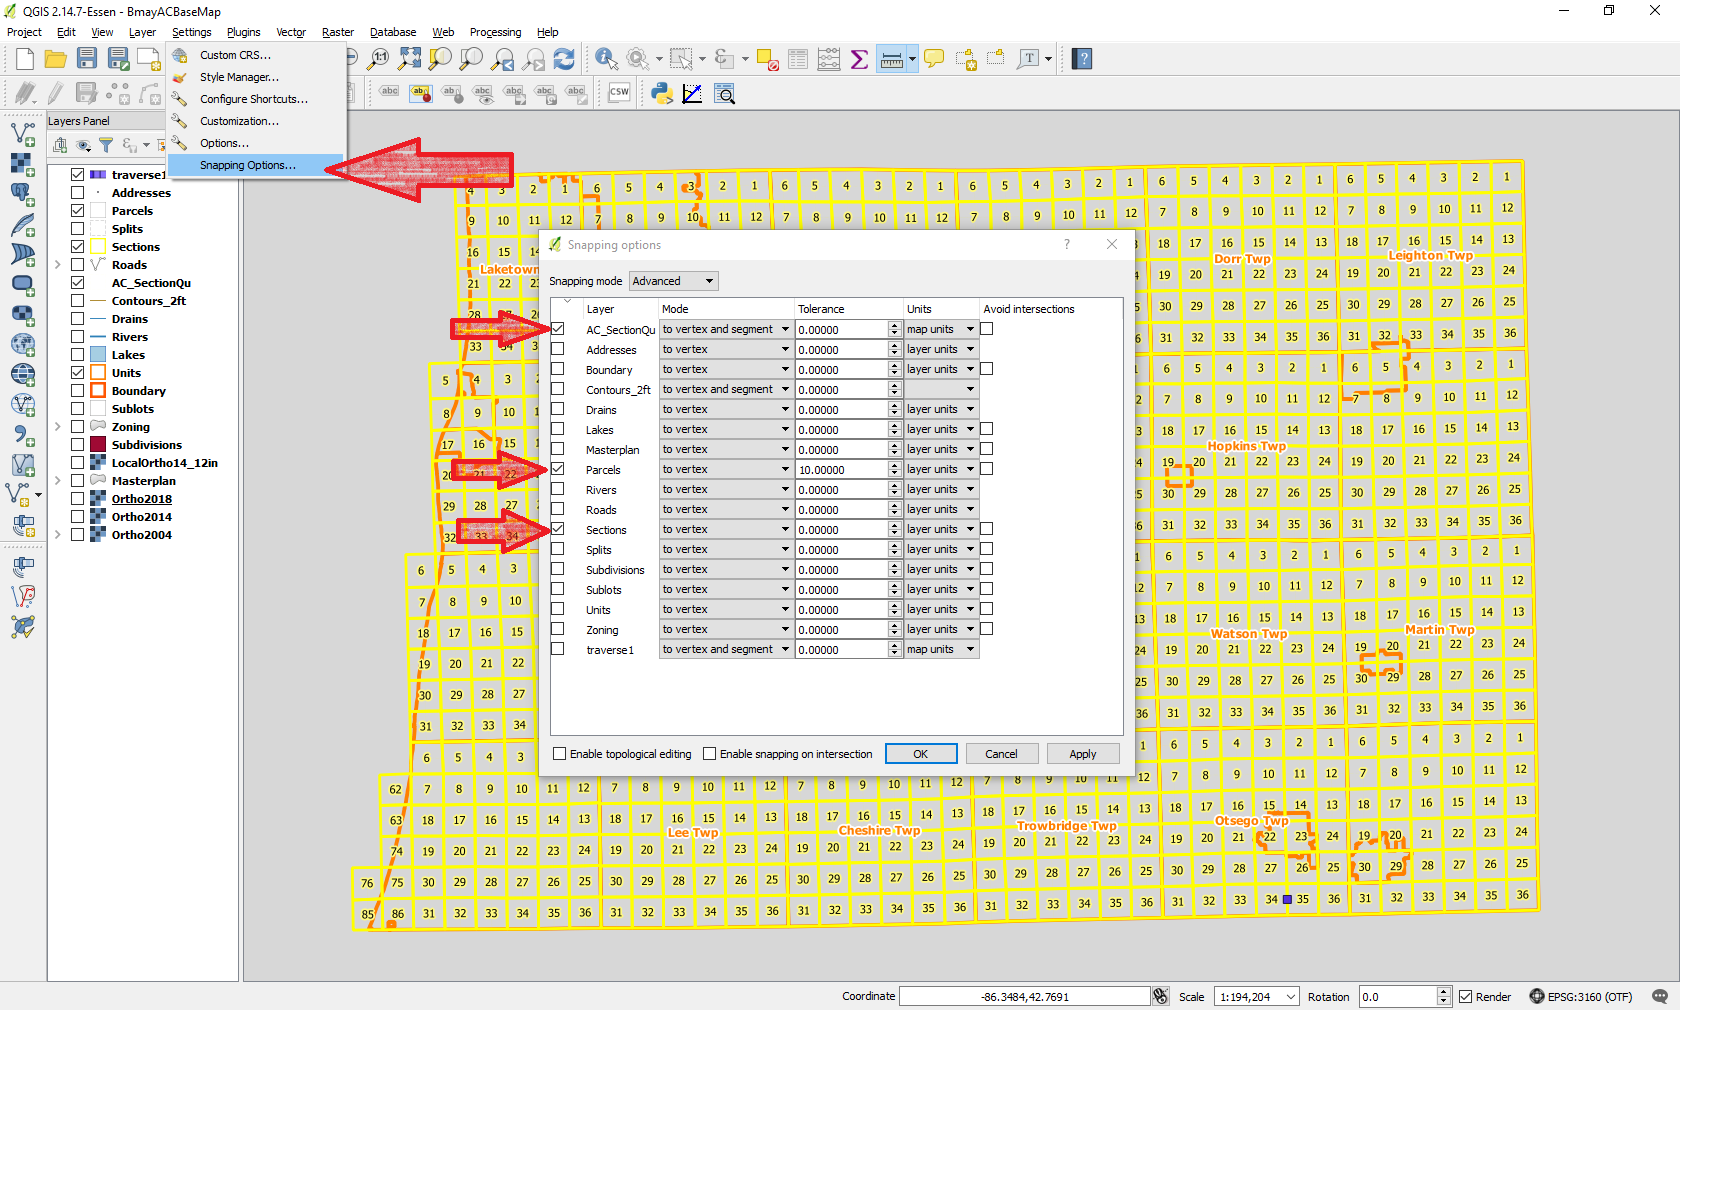
\includegraphics[scale=.3]{7.png} 
	\end{center}
	\caption{Configure editing environment}
\end{figure}
\pagebreak

\subsection{Locate Point of Commencement}
To get to the Point of Commencement,
\medskip

Use \textbf{any combination} of the following methods:
\begin{itemize}
	\item{Using Reference Layer}
	\item{Using Measuring Tool}
	\item{Search by Parcel Number \small(Search Layers Plugin)}
	\item{Draw COGO lines \small(Azd Plugin)}
\end{itemize}

\subsubsection{Using Reference Layer}

{\large Use reference layers; Units, AC\_SectionsQu, Sections, and Parcels.  Toggle layers on and off in Layers Panel and zoom in and out with mouse wheel.}
\pagebreak

\subsubsection{Using Measuring Tool}
\large Use the measuring tool, make sure to set units to feet.  To exit current measurement right click (see fig.).

\end{document}

%\section{Using COGO Tools in QGIS}
%%\pagebreak
%
%\subsection{Set up the Azimuth and Distance Plugin \small(Azd Plugin).}
%%\paragraph{After starting QGIS in the basemap}
%
%\subsubsection{Launch Azd Plugin}
%\large {In the Plugins drop down(1) under the topography group select the Azd Plugin(2)(see fig.).}
%\begin{figure}[H] % included image
%\begin{center}
%%\centering
%	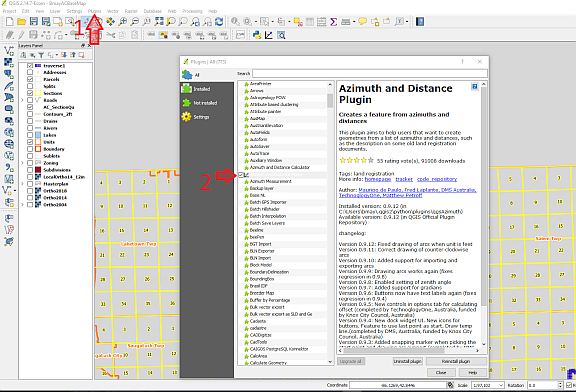
\includegraphics[scale=.25]{1.png}
%	\end{center}
%	\caption{launch plugin}	
%\end{figure}
%%\pagebreak
%\clearpage
%
%\subsubsection{Configure Active Layer}
%\large Note here which layer is active.
%\begin{figure}[H] % included image
%\begin{center}
%	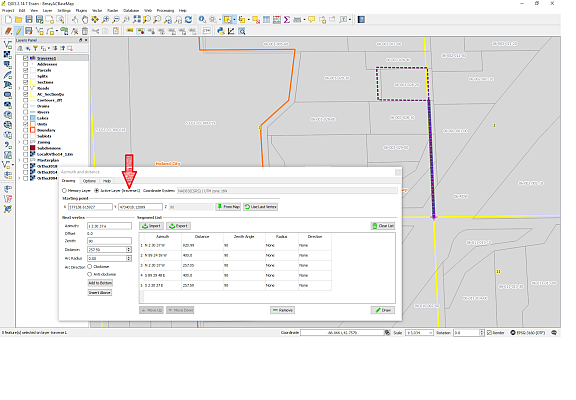
\includegraphics[scale=.2]{2.png} 
%	\end{center}
%	\caption{check active layer}
%\end{figure}
%
%%\noindent
%If necessary, left click the layer traverse 1 in Layer Panel to activate it(see fig.).
%\begin{figure}[H] % Example of including images
%\begin{center}
%	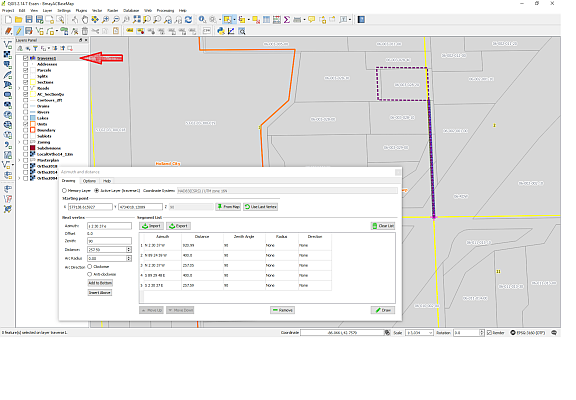
\includegraphics[scale=.2]{3.png} 
%	\end{center}
%	\caption{activate layer}
%\end{figure}
%
%\subsubsection{Configure Options}
%\large On Options Tab: Select Boundary, Bearing, Feet, and Degree radio buttons.
%\begin{figure}[H]
%\begin{center}
%	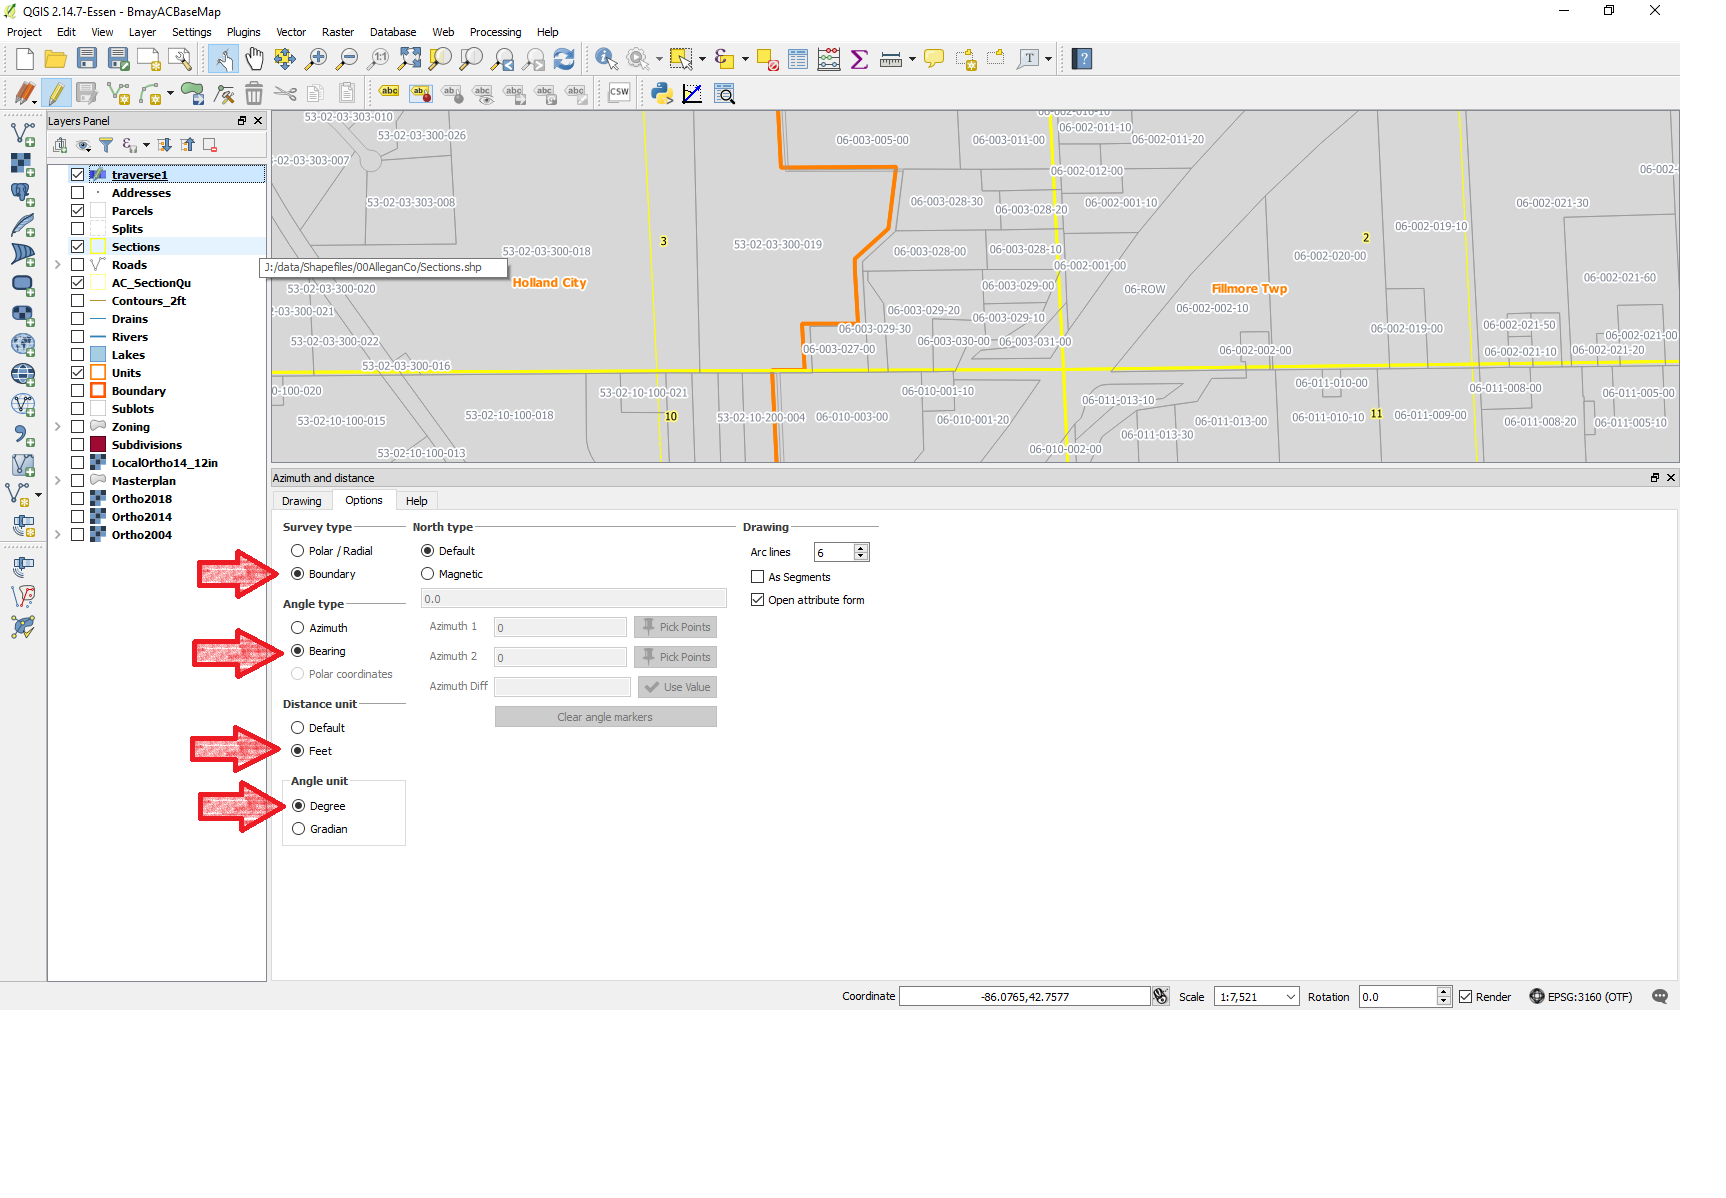
\includegraphics[scale=.3]{4.png} 
%	\end{center}
%	\caption{Plugin Options}
%\end{figure}
%\pagebreak
%
%\subsubsection{Using the tool}
%\large Boundary descriptions are entered into the Drawing Tab. Azimuth (bearing) and Distance are the important boxes (Set Offset = 0 and Zenith = 90 and ignore)(see below).
%\begin{figure}[H]
%\begin{center}
%	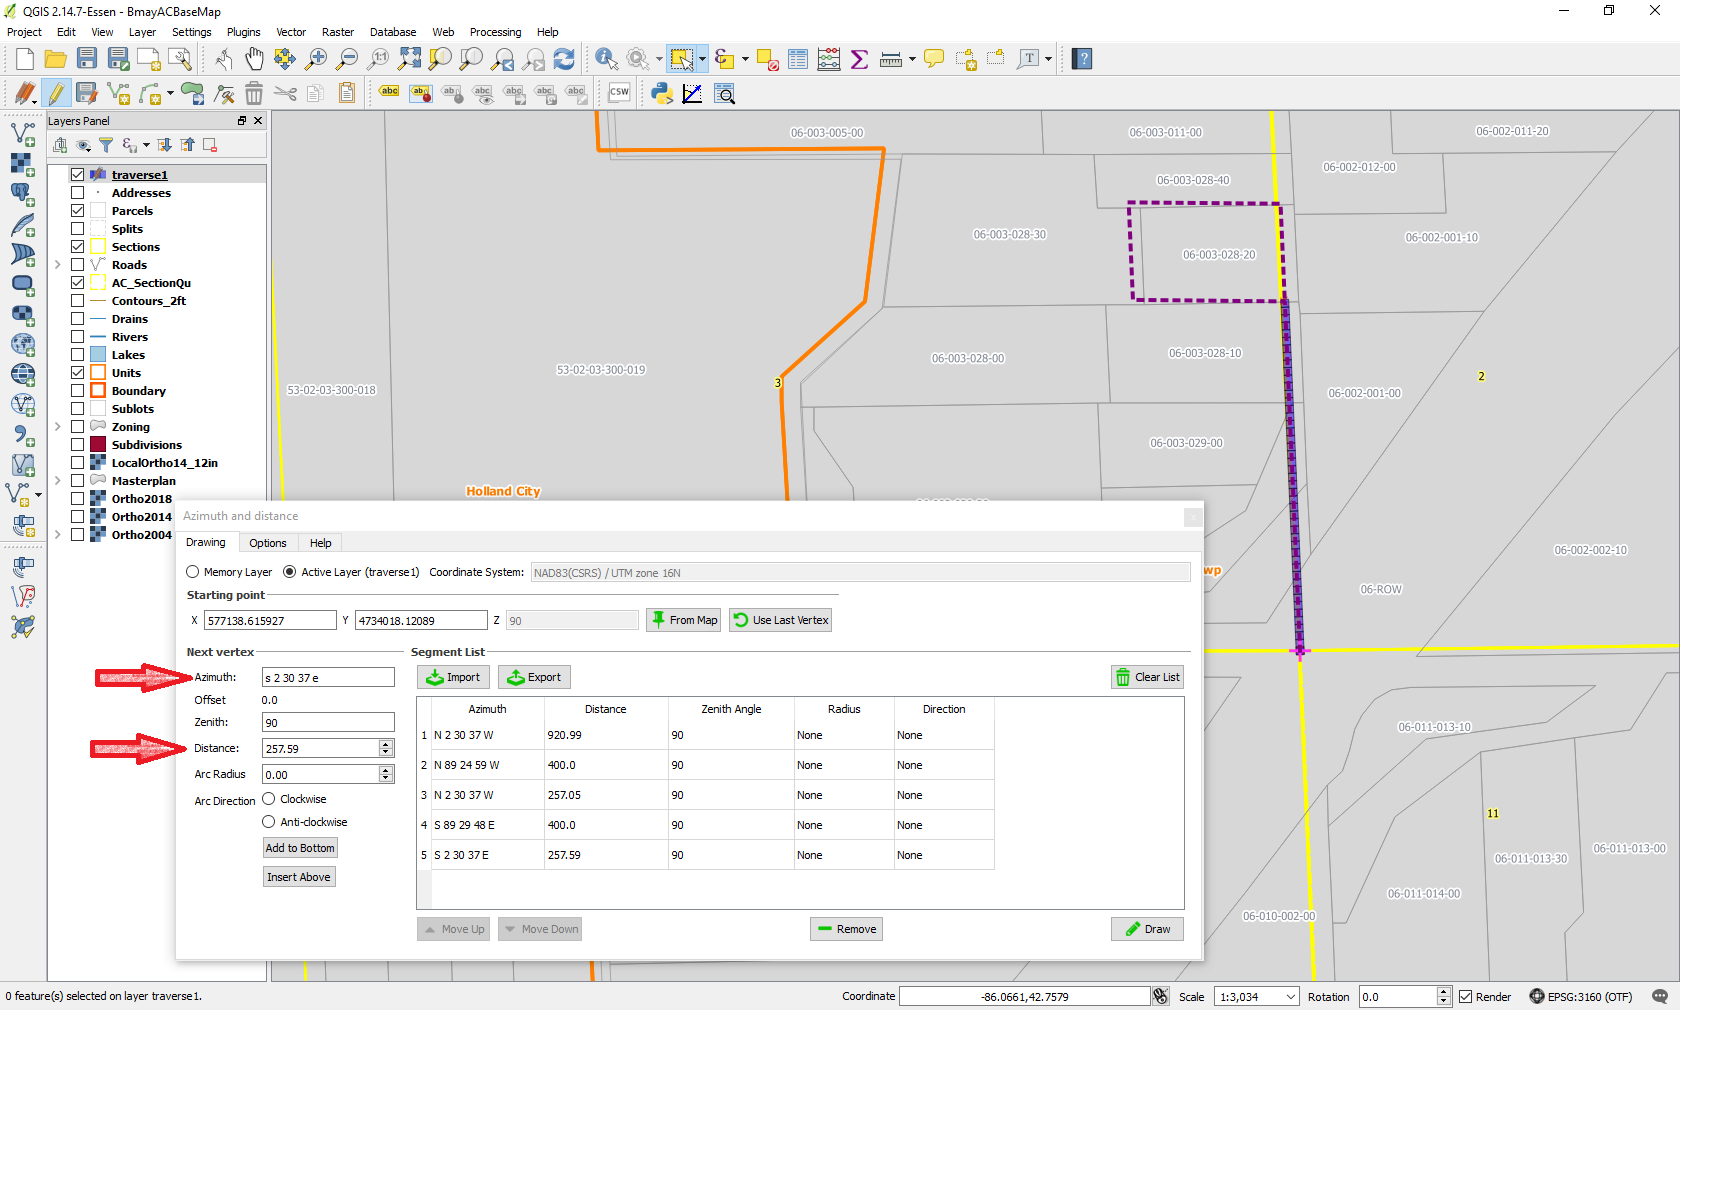
\includegraphics[scale=.3]{5.png} 
%	\end{center}
%	\caption{Entering Bounds}
%\end{figure}
%\pagebreak
%
%\subsection{Configure editing environment}
%\large Use Settings Dropdown and Snapping Options to enable snapping to Sections, Quarter Sections, and or Parcels if desired (see fig.).
%
%\begin{figure}[H]
%\begin{center}
%	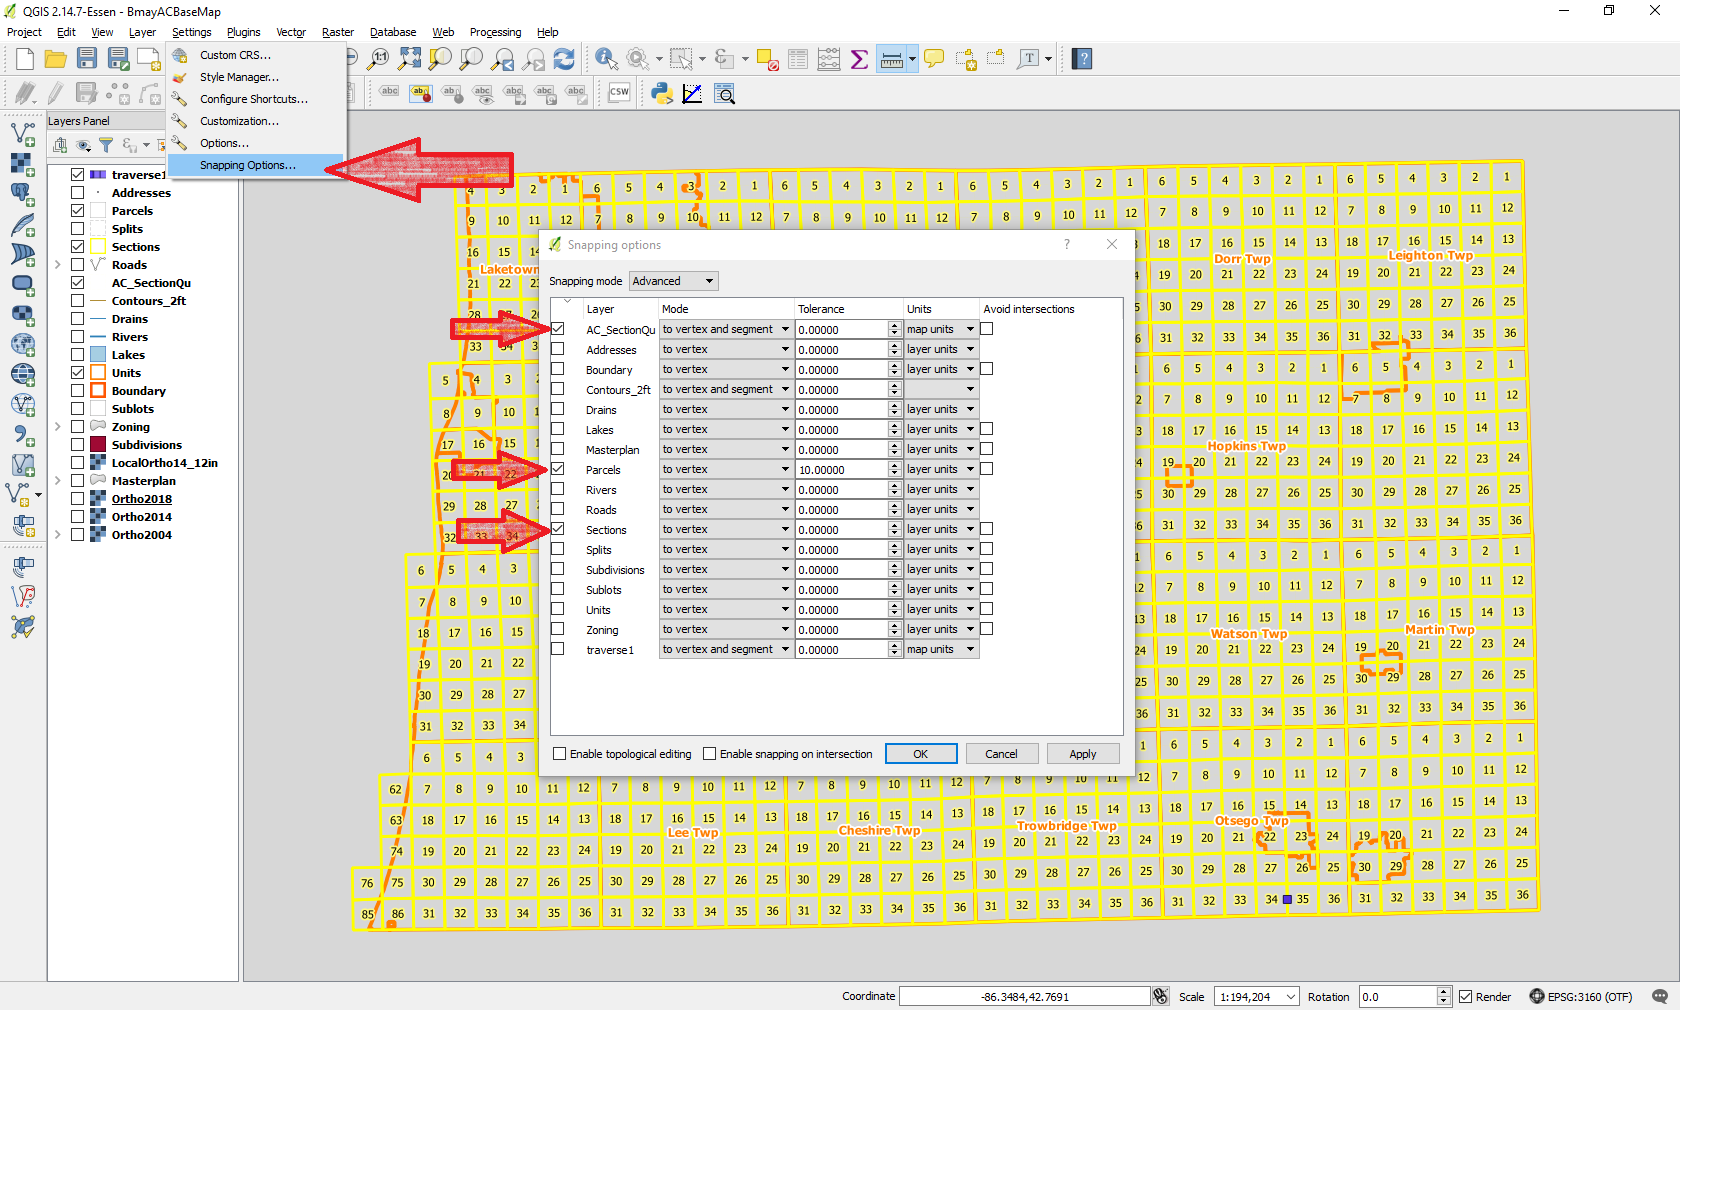
\includegraphics[scale=.3]{7.png} 
%	\end{center}
%	\caption{Configure editing environment}
%\end{figure}
%\pagebreak
%
%\subsection{Locate Point of Commencement}
%To get to the Point of Commencement,
%\medskip
%
%Use \textbf{any combination} of the following methods:
%\begin{itemize}
%	\item{Using Reference Layer}
%	\item{Using Measuring Tool}
%	\item{Search by Parcel Number \small(Search Layers Plugin)}
%	\item{Draw COGO lines \small(Azd Plugin)}
%\end{itemize}
%
%\subsubsection{Using Reference Layer}
%
%{\large Use reference layers; Units, AC\_SectionsQu, Sections, and Parcels.  Toggle layers on and off in Layers Panel and zoom in and out with mouse wheel.}
%\pagebreak
%
%\subsubsection{Using Measuring Tool}
%\large Use the measuring tool, make sure to set units to feet.  To exit current measurement right click (see fig.).
%
%\begin{figure}[H]
%\begin{center}
%	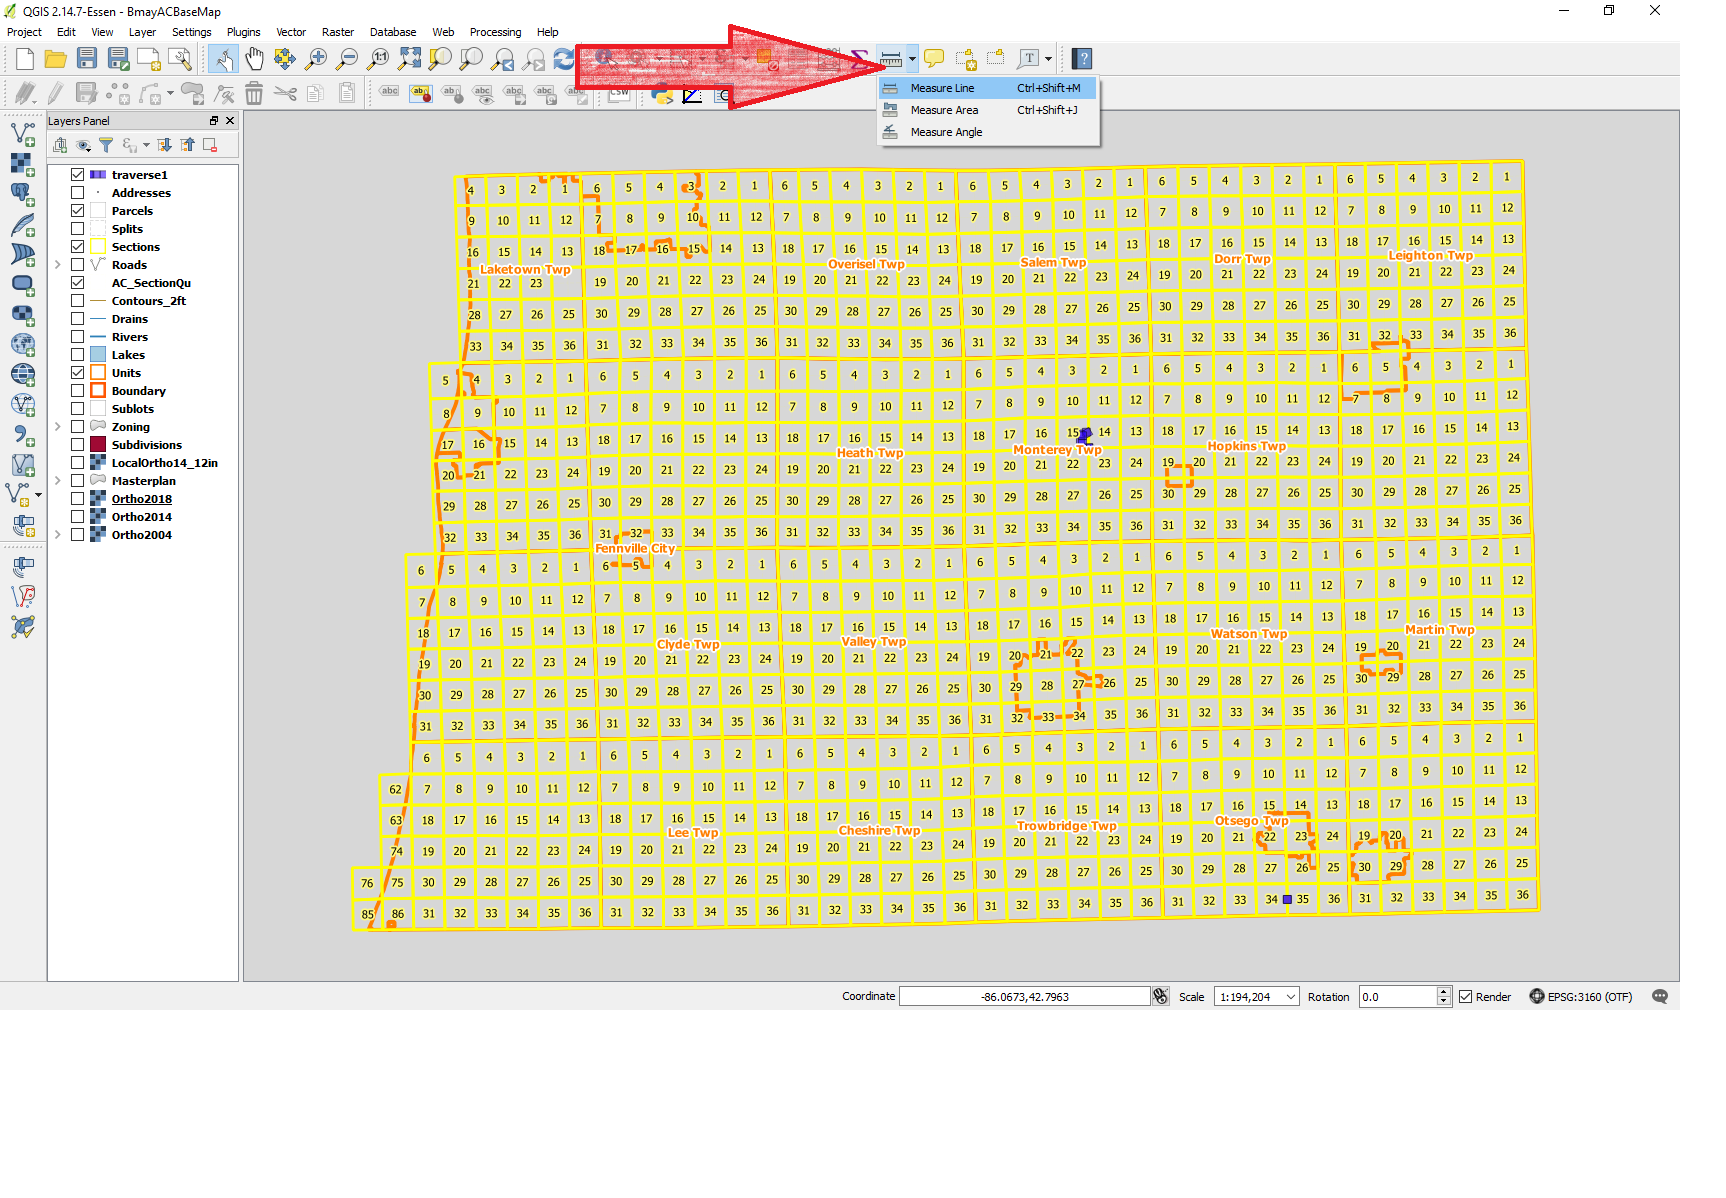
\includegraphics[scale=.3]{6.png} 
%	\end{center}
%	\caption{Measure Tool}
%\end{figure}
%\pagebreak
%
%\subsubsection{Search by Parcel Number \small(Launch Search Layers Plugin)}
%In the \underline{Plugins} drop down:\\\\ select the \textbf{Search Layers Plugin}(see fig.).
%\begin{figure}[H] % included image
%\begin{center}
%%\centering
%	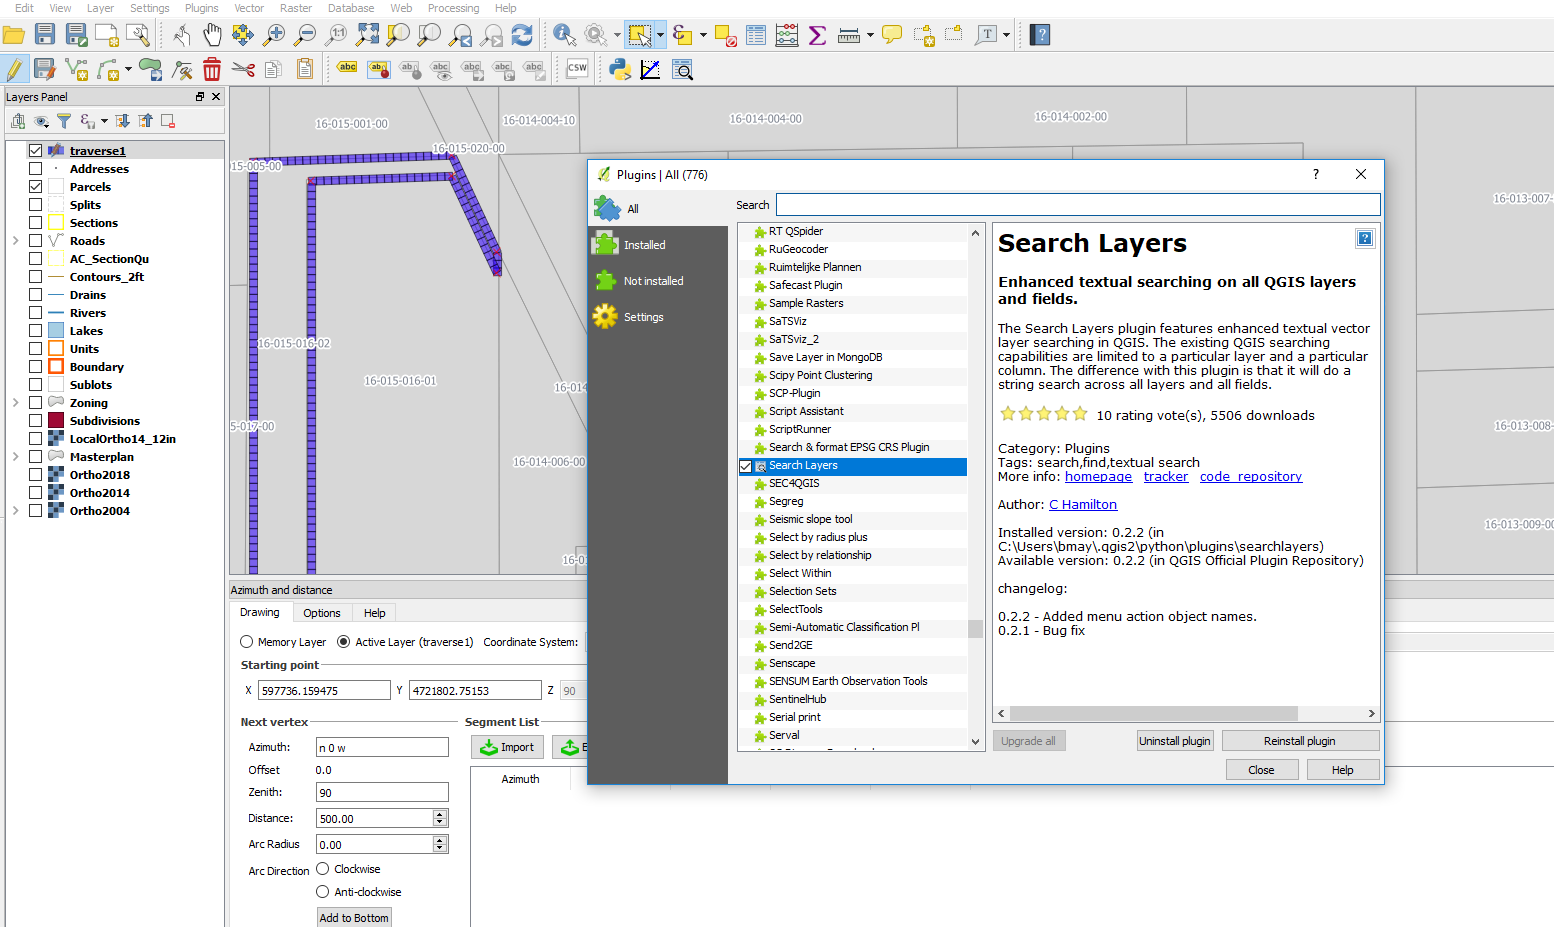
\includegraphics[scale=.3]{SearchLayers1b.png}
%	\end{center}
%	\caption{launch plugin}	
%\end{figure}
%\pagebreak
%
%\subsubsection{Use Search Layers Plugin}
%
%For \underline{Search String}:\\\\Type parcel numbers with dashes ie. \textbf{\textit{16-015-016-10}}.\\\\Set \underline{Search Layers} to \textbf{\textit{Parcels}}\\\\ and \underline{Search Fields} to \textbf{\textit{PARCELID}}\\\\Press Search button.\\\\Click on a result to zoom to parcel(see fig.).
%
%\begin{figure}[H]
%\begin{center}
%	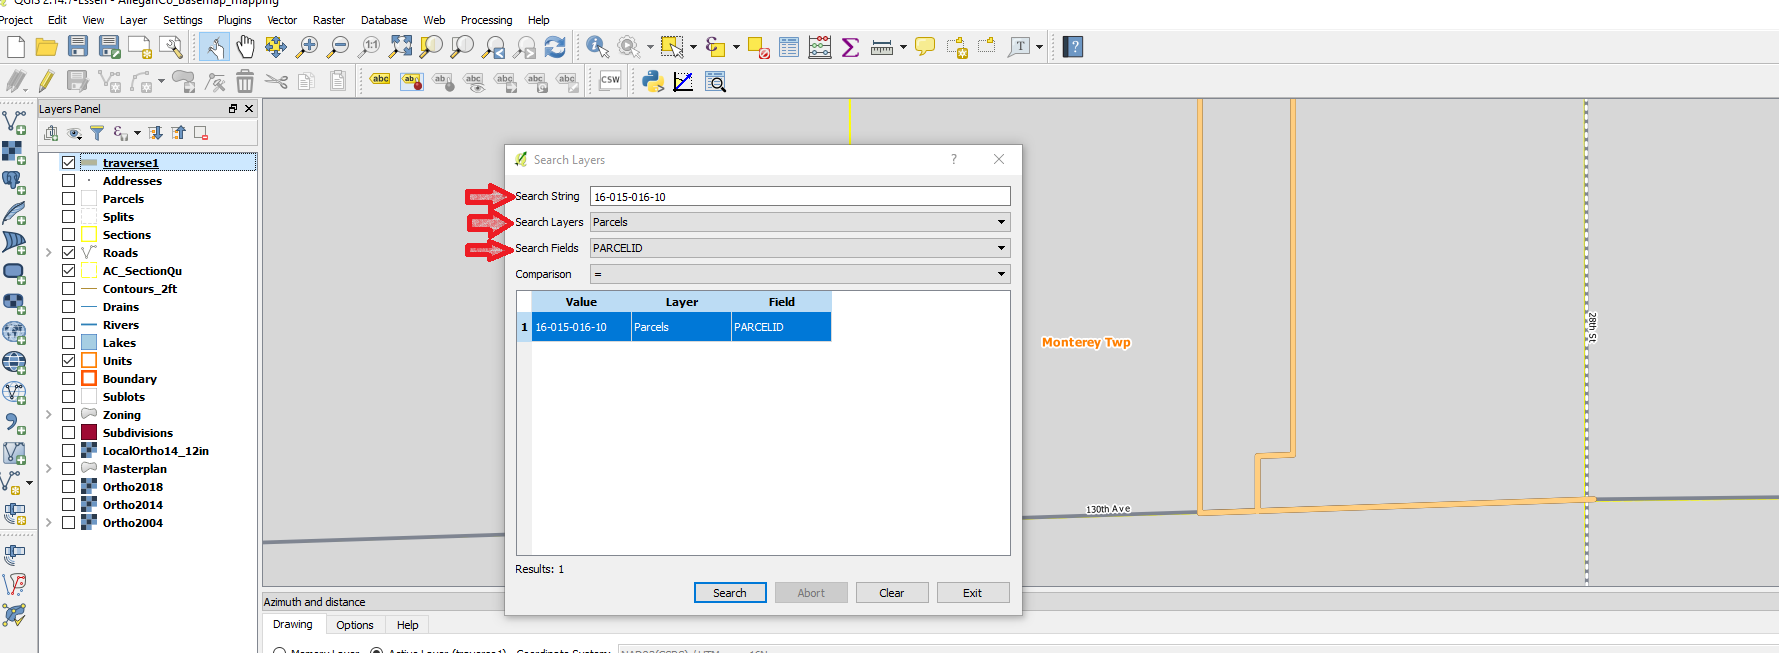
\includegraphics[scale=.35]{SearchLayers.png} 
%	\end{center}
%	\caption{Parcel Search}
%\end{figure}
%\pagebreak
%
%\subsubsection{Use COGO}
%Launch and Configure Azd Plugin as described in 1.1.\\\\Enter line bearings and distances into the Azd Plugin to get from a known point or Point of Commencement to the Point of Beginning.\\\\Use the Drawing Tab of AzD Plugin.\\\\Tab between Azimuth and Distance and then click on Add to Bottom(Note: Offset = 0 and Zenith = 90)(see fig.).\\\\For first segment: press the From Map button and select point of beginning on the map.\\\\Push Draw button to draw segment list to traverse1.
%\begin{figure}[H]
%\begin{center}
%	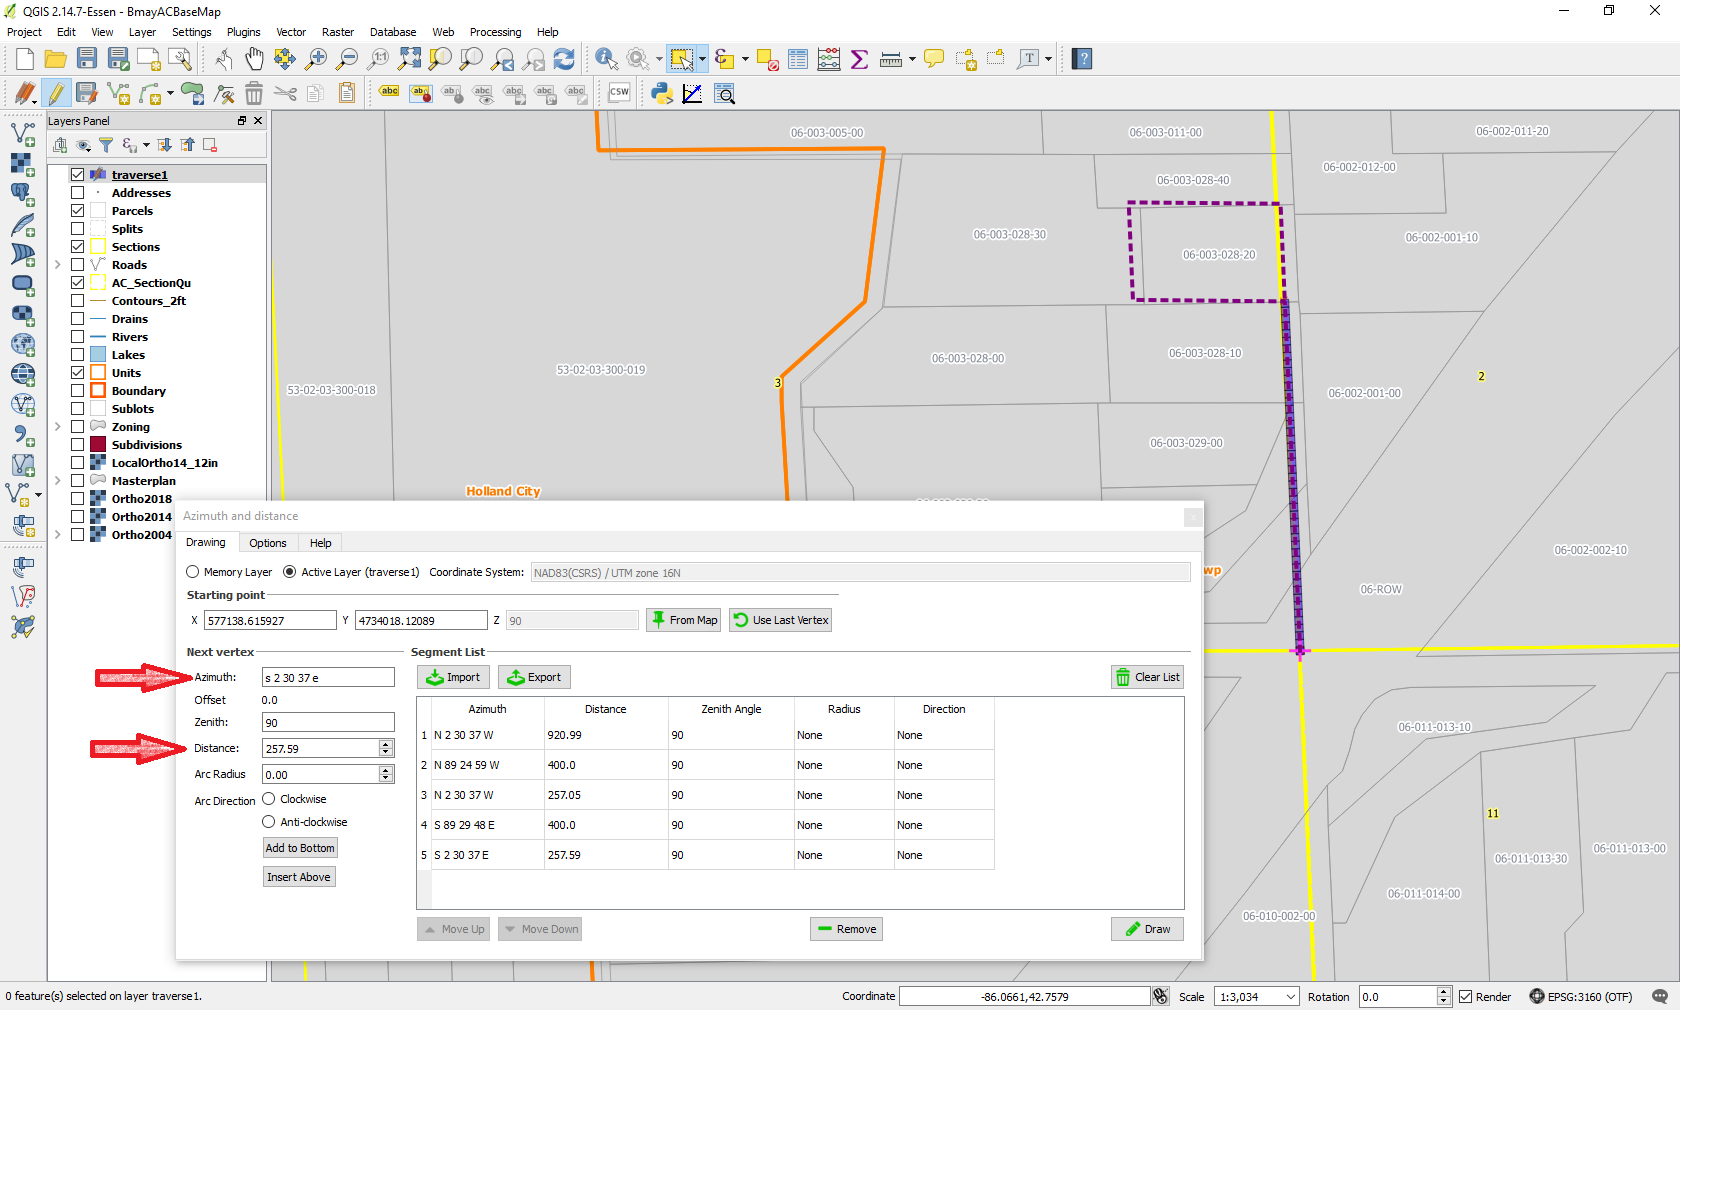
\includegraphics[scale=.25]{5.png} 
%	\end{center}
%	\caption{Entering Bearing and Distance}
%\end{figure}
%\pagebreak
%
%\subsection{Drawing parcel}
%\subsubsection{Enter Description} 
%\large Enter Metes and Bounds Boundary description from Point of Beginning onward into Drawing Tab of AzD Plugin.\\\\Tab between Azimuth and Distance and then click on Add to Bottom to assemble Segment List.\\\small Order of segments can be changed with move up and move down buttons.\\\\Push Use Last Vertex button to get to Point of Beginning.\\\\Press Draw to draw parcel(see fig.).
%
%\begin{figure}[H]
%\begin{center}
%	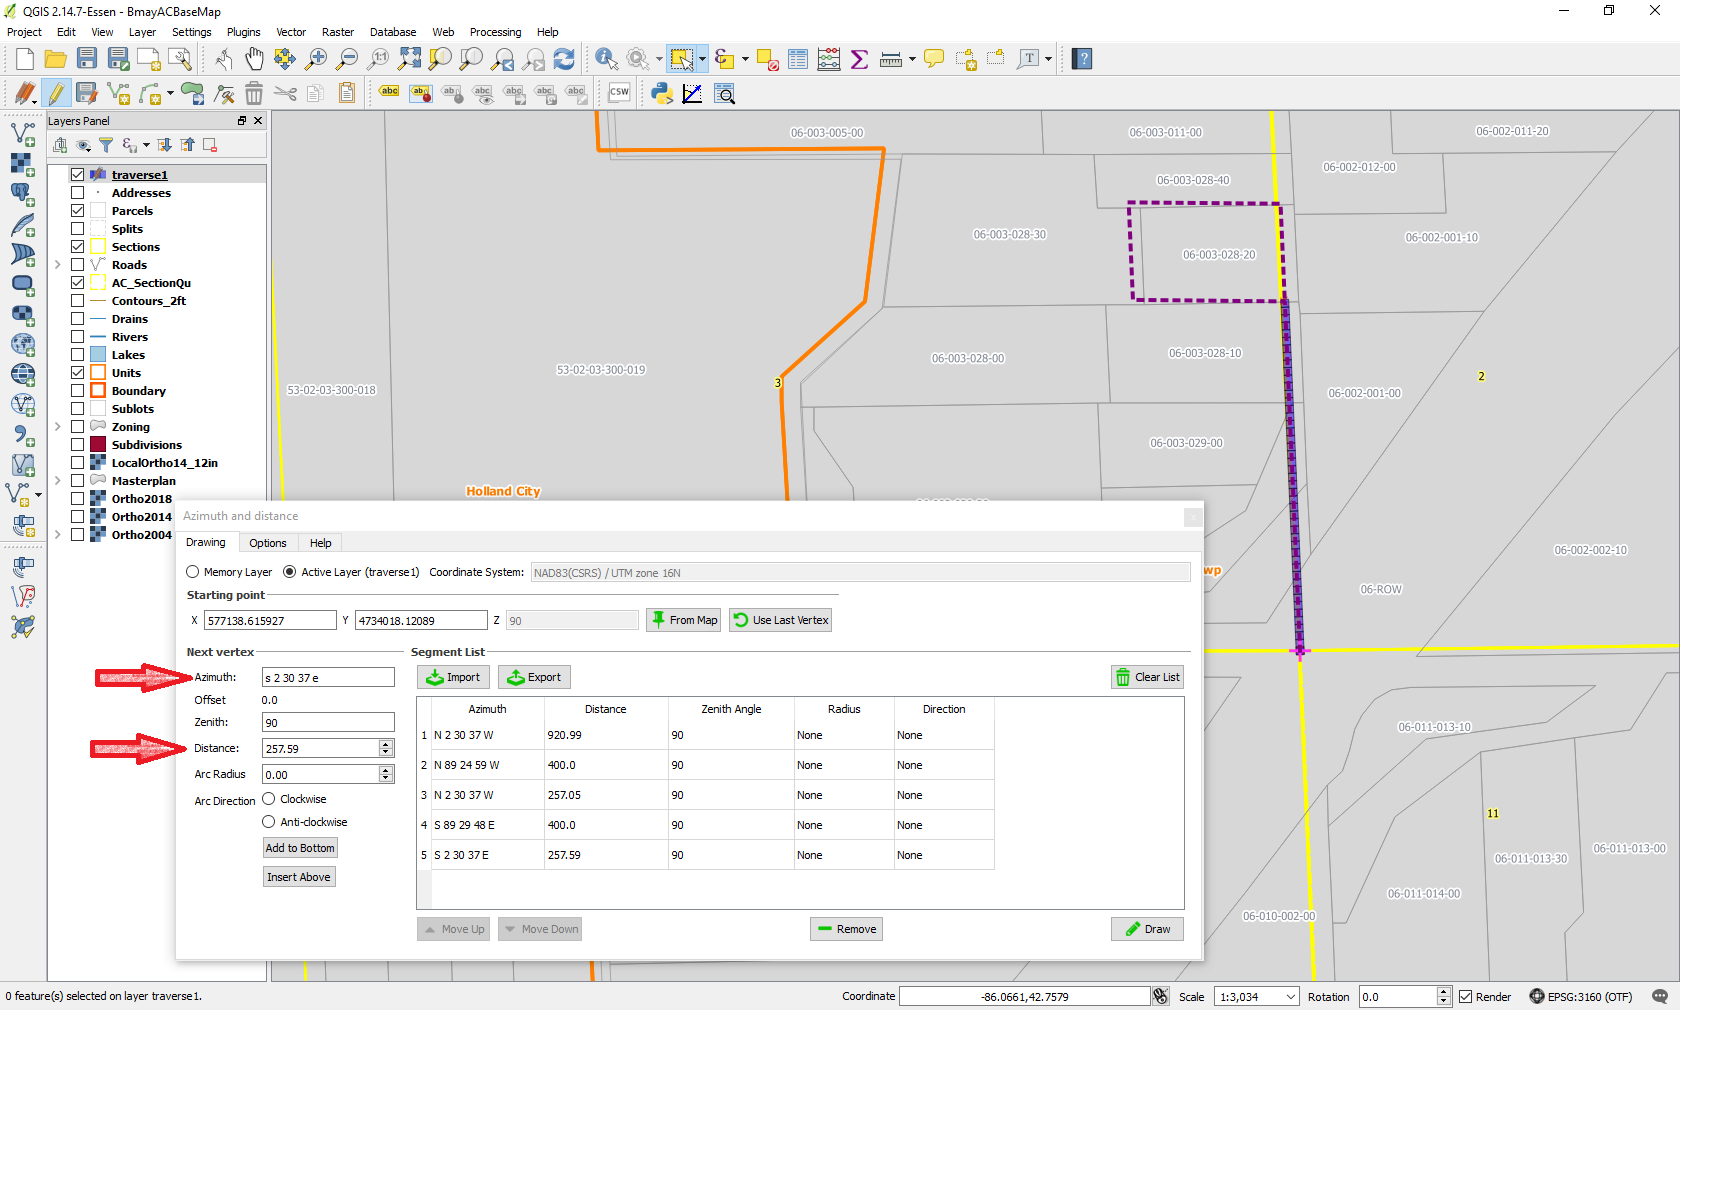
\includegraphics[scale=.3]{5.png} 
%	\end{center}
%	\caption{Entering Bearing and Distance}
%\end{figure}
%
%\pagebreak

\end{document}
 
 
 
